%FELSENSTEIN'S LIKELIHOOD
\begin{frame}[plain]
\frametitle{Felsenstein's likelihood (1981)}

\begin{columns}[t]

\column{.64\textwidth}

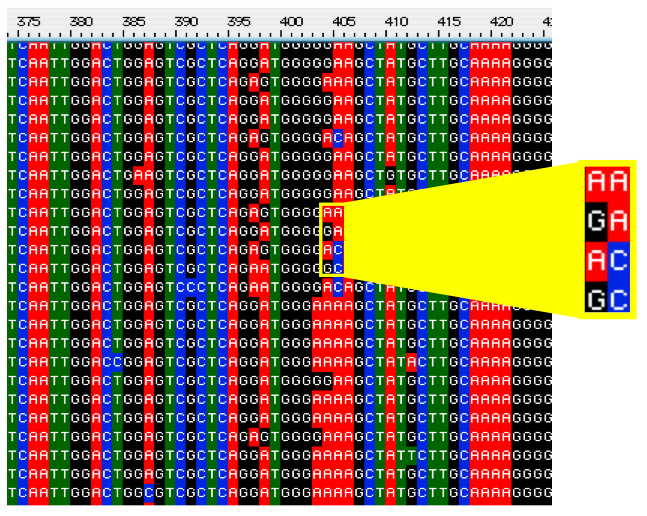
\includegraphics[width=\textwidth]{../images/MolecularEvolModel1}

\column{.36\textwidth}

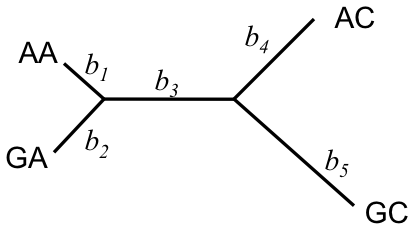
\includegraphics[width=0.9\textwidth]{../images/MolecularEvolModel2}

\smallskip{}

$L(T) = Pr\{D|T,Q\}$

\medskip{}

\scriptsize{
The probability of the data, \textbf{$Pr\{D|T,Q\}$} can be efficiently calculated given a phylogenetic tree ($T$), and a \textbf{probabilistic model} of molecular evolution ($Q$). 

\medskip{}

\textbf{In statistical phylogenetics, branch lengths are traditionally unconstrained}.
}

\end{columns}

\end{frame}
